%Notes by Harsh Mistry 
%CS 349
%Based on Template From  https://www.cs.cmu.edu/~ggordon/10725-F12/template.tex

\documentclass[twoside]{article}
\setlength{\oddsidemargin}{0.25 in}
\setlength{\evensidemargin}{-0.25 in}
\setlength{\topmargin}{-0.6 in}
\setlength{\textwidth}{6.5 in}
\setlength{\textheight}{8.5 in}
\setlength{\headsep}{0.75 in}
\setlength{\parindent}{0 in}
\setlength{\parskip}{0.1 in}
\usepackage{amsmath,amsfonts,graphicx}
\newcounter{lecnum}
\renewcommand{\thepage}{\thelecnum-\arabic{page}}
\renewcommand{\thesection}{\thelecnum.\arabic{section}}
\renewcommand{\theequation}{\thelecnum.\arabic{equation}}
\renewcommand{\thefigure}{\thelecnum.\arabic{figure}}
\renewcommand{\thetable}{\thelecnum.\arabic{table}}
\newcommand{\lecture}[4]{
   \pagestyle{myheadings}
   \thispagestyle{plain}
   \newpage
   \setcounter{lecnum}{#1}
   \setcounter{page}{1}
   
   
%Info Box 
   \begin{center}
   \framebox{
      \vbox{\vspace{2mm}
    \hbox to 6.28in { {\bf CS 349 - User Interfaces
	\hfill Winter 2018} }
       \vspace{4mm}
       \hbox to 6.28in { {\Large \hfill Lecture #1: #2  \hfill} }
       \vspace{2mm}
       \hbox to 6.28in { {\it Lecturer: #3 \hfill Notes By: #4} }
      \vspace{2mm}}
   }
   \end{center}
   
   \markboth{Lecture #1: #2}{Lecture #1: #2}



 
}

\renewcommand{\cite}[1]{[#1]}
\def\beginrefs{\begin{list}%
        {[\arabic{equation}]}{\usecounter{equation}
         \setlength{\leftmargin}{2.0truecm}\setlength{\labelsep}{0.4truecm}%
         \setlength{\labelwidth}{1.6truecm}}}
\def\endrefs{\end{list}}
\def\bibentry#1{\item[\hbox{[#1]}]}

\newcommand{\fig}[3]{
			\vspace{#2}
			\begin{center}
			Figure \thelecnum.#1:~#3
			\end{center}
	}
	
\graphicspath{ {images/} }

\newtheorem{theorem}{Theorem}[lecnum]
\newtheorem{lemma}[theorem]{Lemma}
\newtheorem{ex}[theorem]{Example}
\newtheorem{proposition}[theorem]{Proposition}
\newtheorem{claim}[theorem]{Claim}
\newtheorem{corollary}[theorem]{Corollary}
\newtheorem{definition}[theorem]{Definition}
\newenvironment{proof}{{\bf Proof:}}{\hfill\rule{2mm}{2mm}}
\newcommand\E{\mathbb{E}}


%Start of Document 
\begin{document}

\lecture{3}{January 8, 2018}{Keiko Katsuragawa}{Harsh Mistry}

\section{Windowing Systems}
\subsection{Windowing System}
\begin{itemize}
\item Handles input device events
\item Exposes output methods to display graphics
\begin{itemize}
\item basic drawing primitives, bitmaps, text
\end{itemize}
\item Manages windows as a place for visual application content 
\item A \textbf{windowing system} provides "low-level" input, output, and window management capabilities to the operating system. 
\end{itemize}

\subsection{X windows}
\begin{itemize}
\item Developed in 1984
\item Standard windowing system for Unixes
\item Free and Cross-Platform
\item Unix standard windowing system 
\begin{itemize}
\item handles input, draws graphics, create windows, ...
\item free and cross-platform 
\end{itemize}
\item Essentially a protocol
\begin{itemize}
\item does not specify style of user interface
\item not a "window manager" 

\item A windowing system provides "low-level" input, output and window management capabilities to the operating systems 
\end{itemize}
\end{itemize}

\subsubsection{X Windows Design Criteria}
\begin{itemize}
\item Implementable on a variety of displays
\item Applications must be device independent
\item Must be network transparent
\item Support multiple, concurrent application displays
\item Support output to overlapping windows (... even when partially obscured)
\item Support a hierarchy of resizeable windows
\item Support many different applications
\item High-performance, high-quality text, 2-D graphics, imaging .. 
\item System should be extensible
\end{itemize}

\subsubsection{X Client Server Architecture}
\begin{itemize}
\item An X Client handles all application logic 
\item An X server handles all display output and user input
\item Server handles request from client, process data as requested, and returns results to client
\end{itemize}

\subsubsection{Why Client-Server?}
\begin{itemize}
\item Goal was flexibility and economy 
\item Many X clients can exist, while only one X server delvers the user interface 
\end{itemize}

\begin{center}
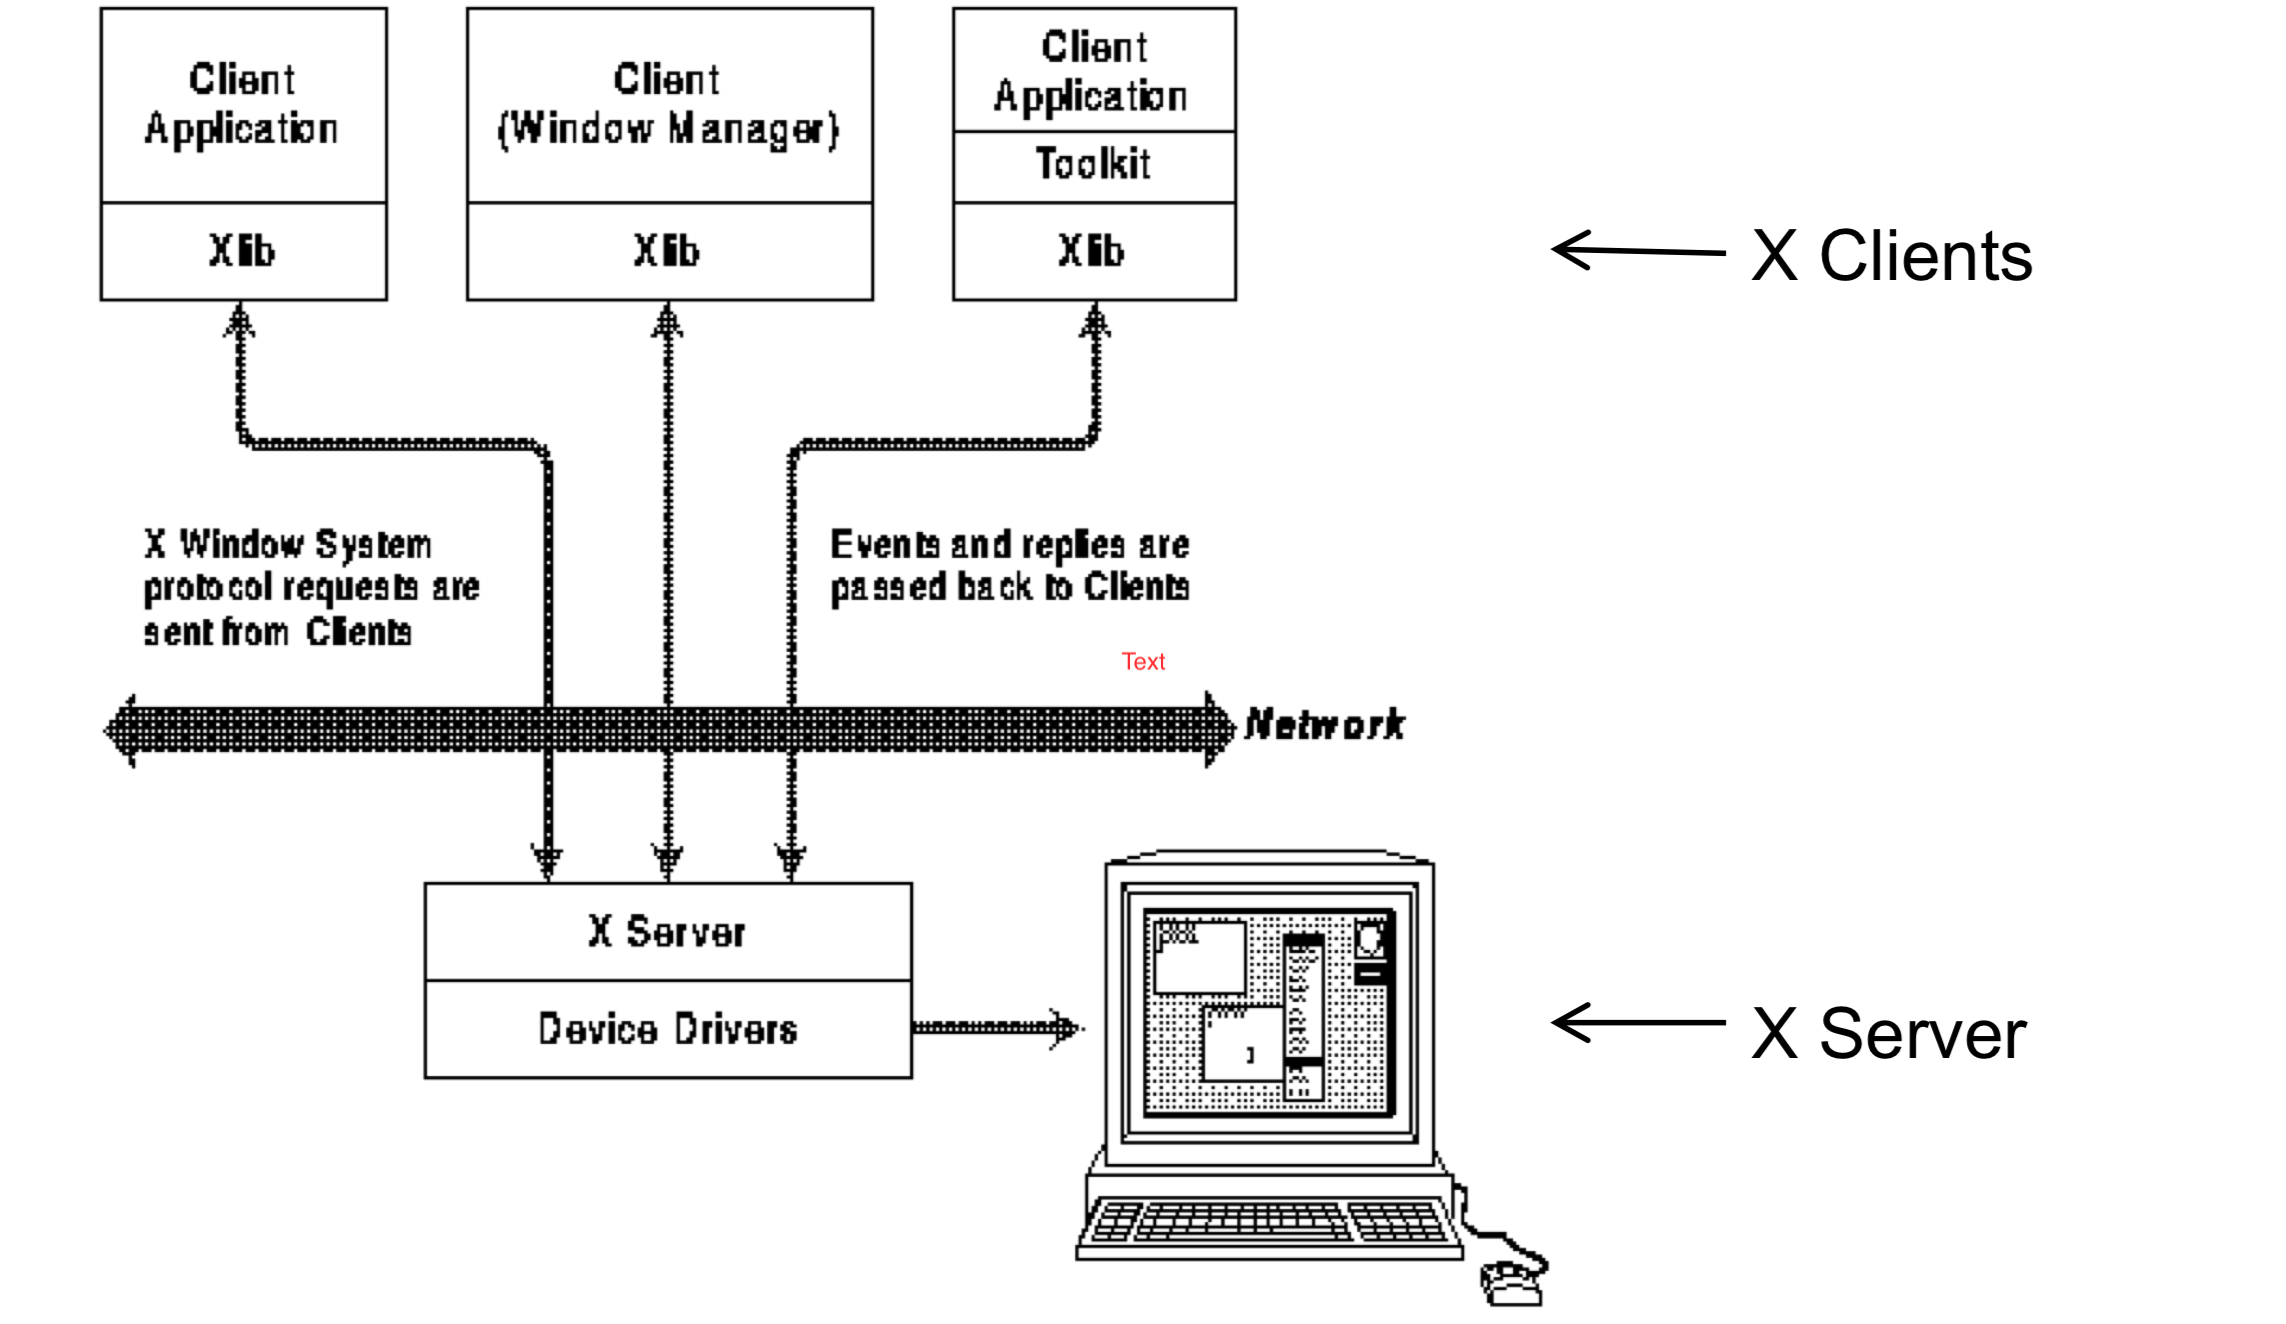
\includegraphics[scale=0.3]{1}
\end{center}
\newpage
\subsubsection{Structure of a typical X program}
\begin{itemize}
\item Perform X Client initialization
\item Connect to the X server
\item Perform X related initialization 
\item Event loop \\
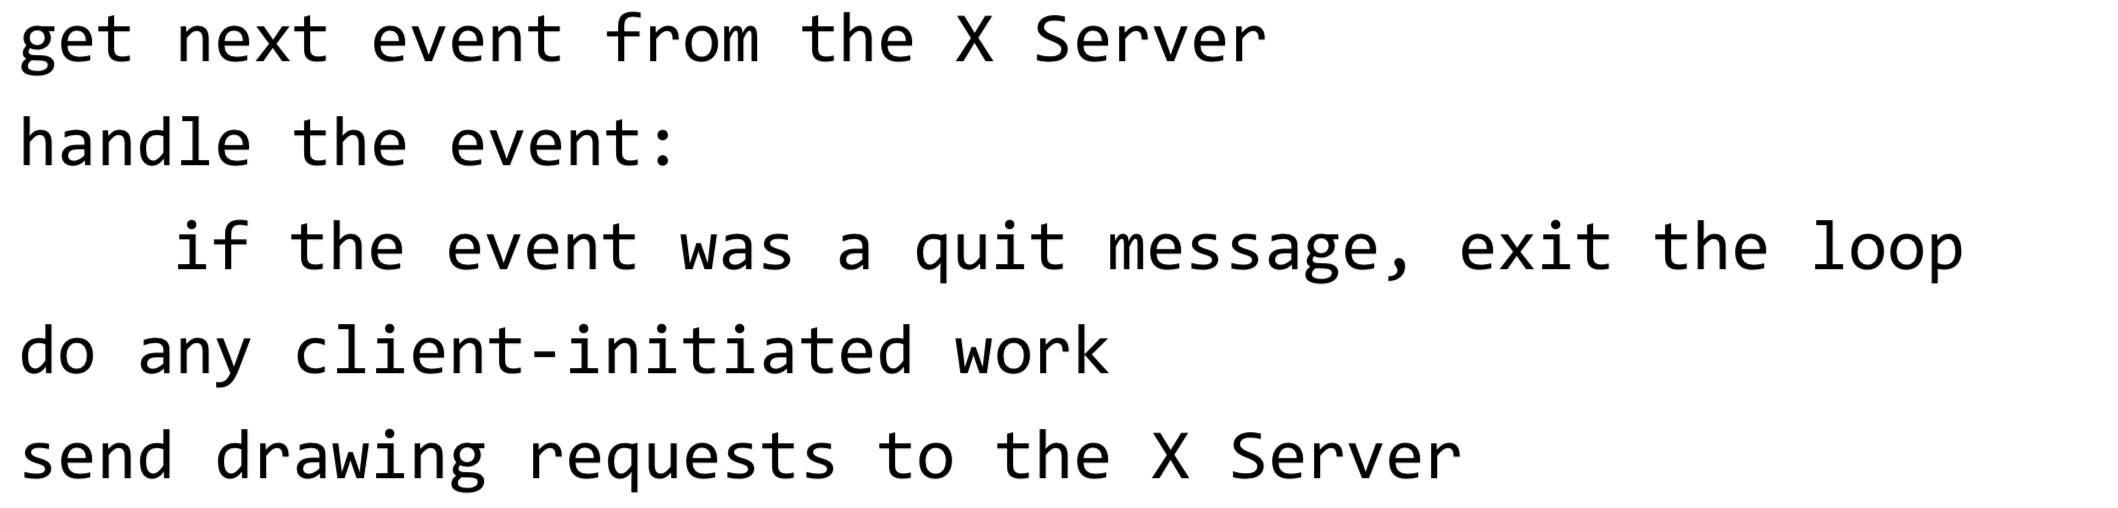
\includegraphics[scale=0.3]{2}
\item close down the connection to the X Server
\item perform client cleanup
\end{itemize}

\subsubsection{Xlib}
\begin{itemize}
\item library to wrap low level X Window protocol
\begin{itemize}
\item to avoid implementing message passing for every new program
\end{itemize}
\item uses buffered input and output queues 
\begin{itemize}
\item need to flush them: XSync, XFlush
\end{itemize}
\item Xlib functions:
\begin{itemize}
\item connection operations: e.g. XOpenDisplay, XCloseDisplay, ...
\item connection operation requests: e.g. XCreateWindow, XCreateGC,...
\item connection information requests: e.g. XGetWindowProperty, ...
\item local event queue operations: e.g. XNextEvent, XPeekEvent, ...
\item local data operations: e.g. XLookupKeysym, XParseGeometry, XSetRegion, XCreateImage, XSaveContext, ...
\end{itemize}
\item Xlib data types:
\begin{itemize}
\item Display, Window, GC, XSizeHints, XWhitePixel, XBlackPixel, etc.
\end{itemize} 
\end{itemize}

\subsubsection{Compile and run an X application}
\verb|g++ -o null null.cpp -L/usr/X11R6/lib -lX11 -lstdc++ ./null|

\subsubsection{Sample Code}
Refer to Pages 14-16 of course slides for code examples 

\subsection{Windowing System Architecture}
\begin{center}
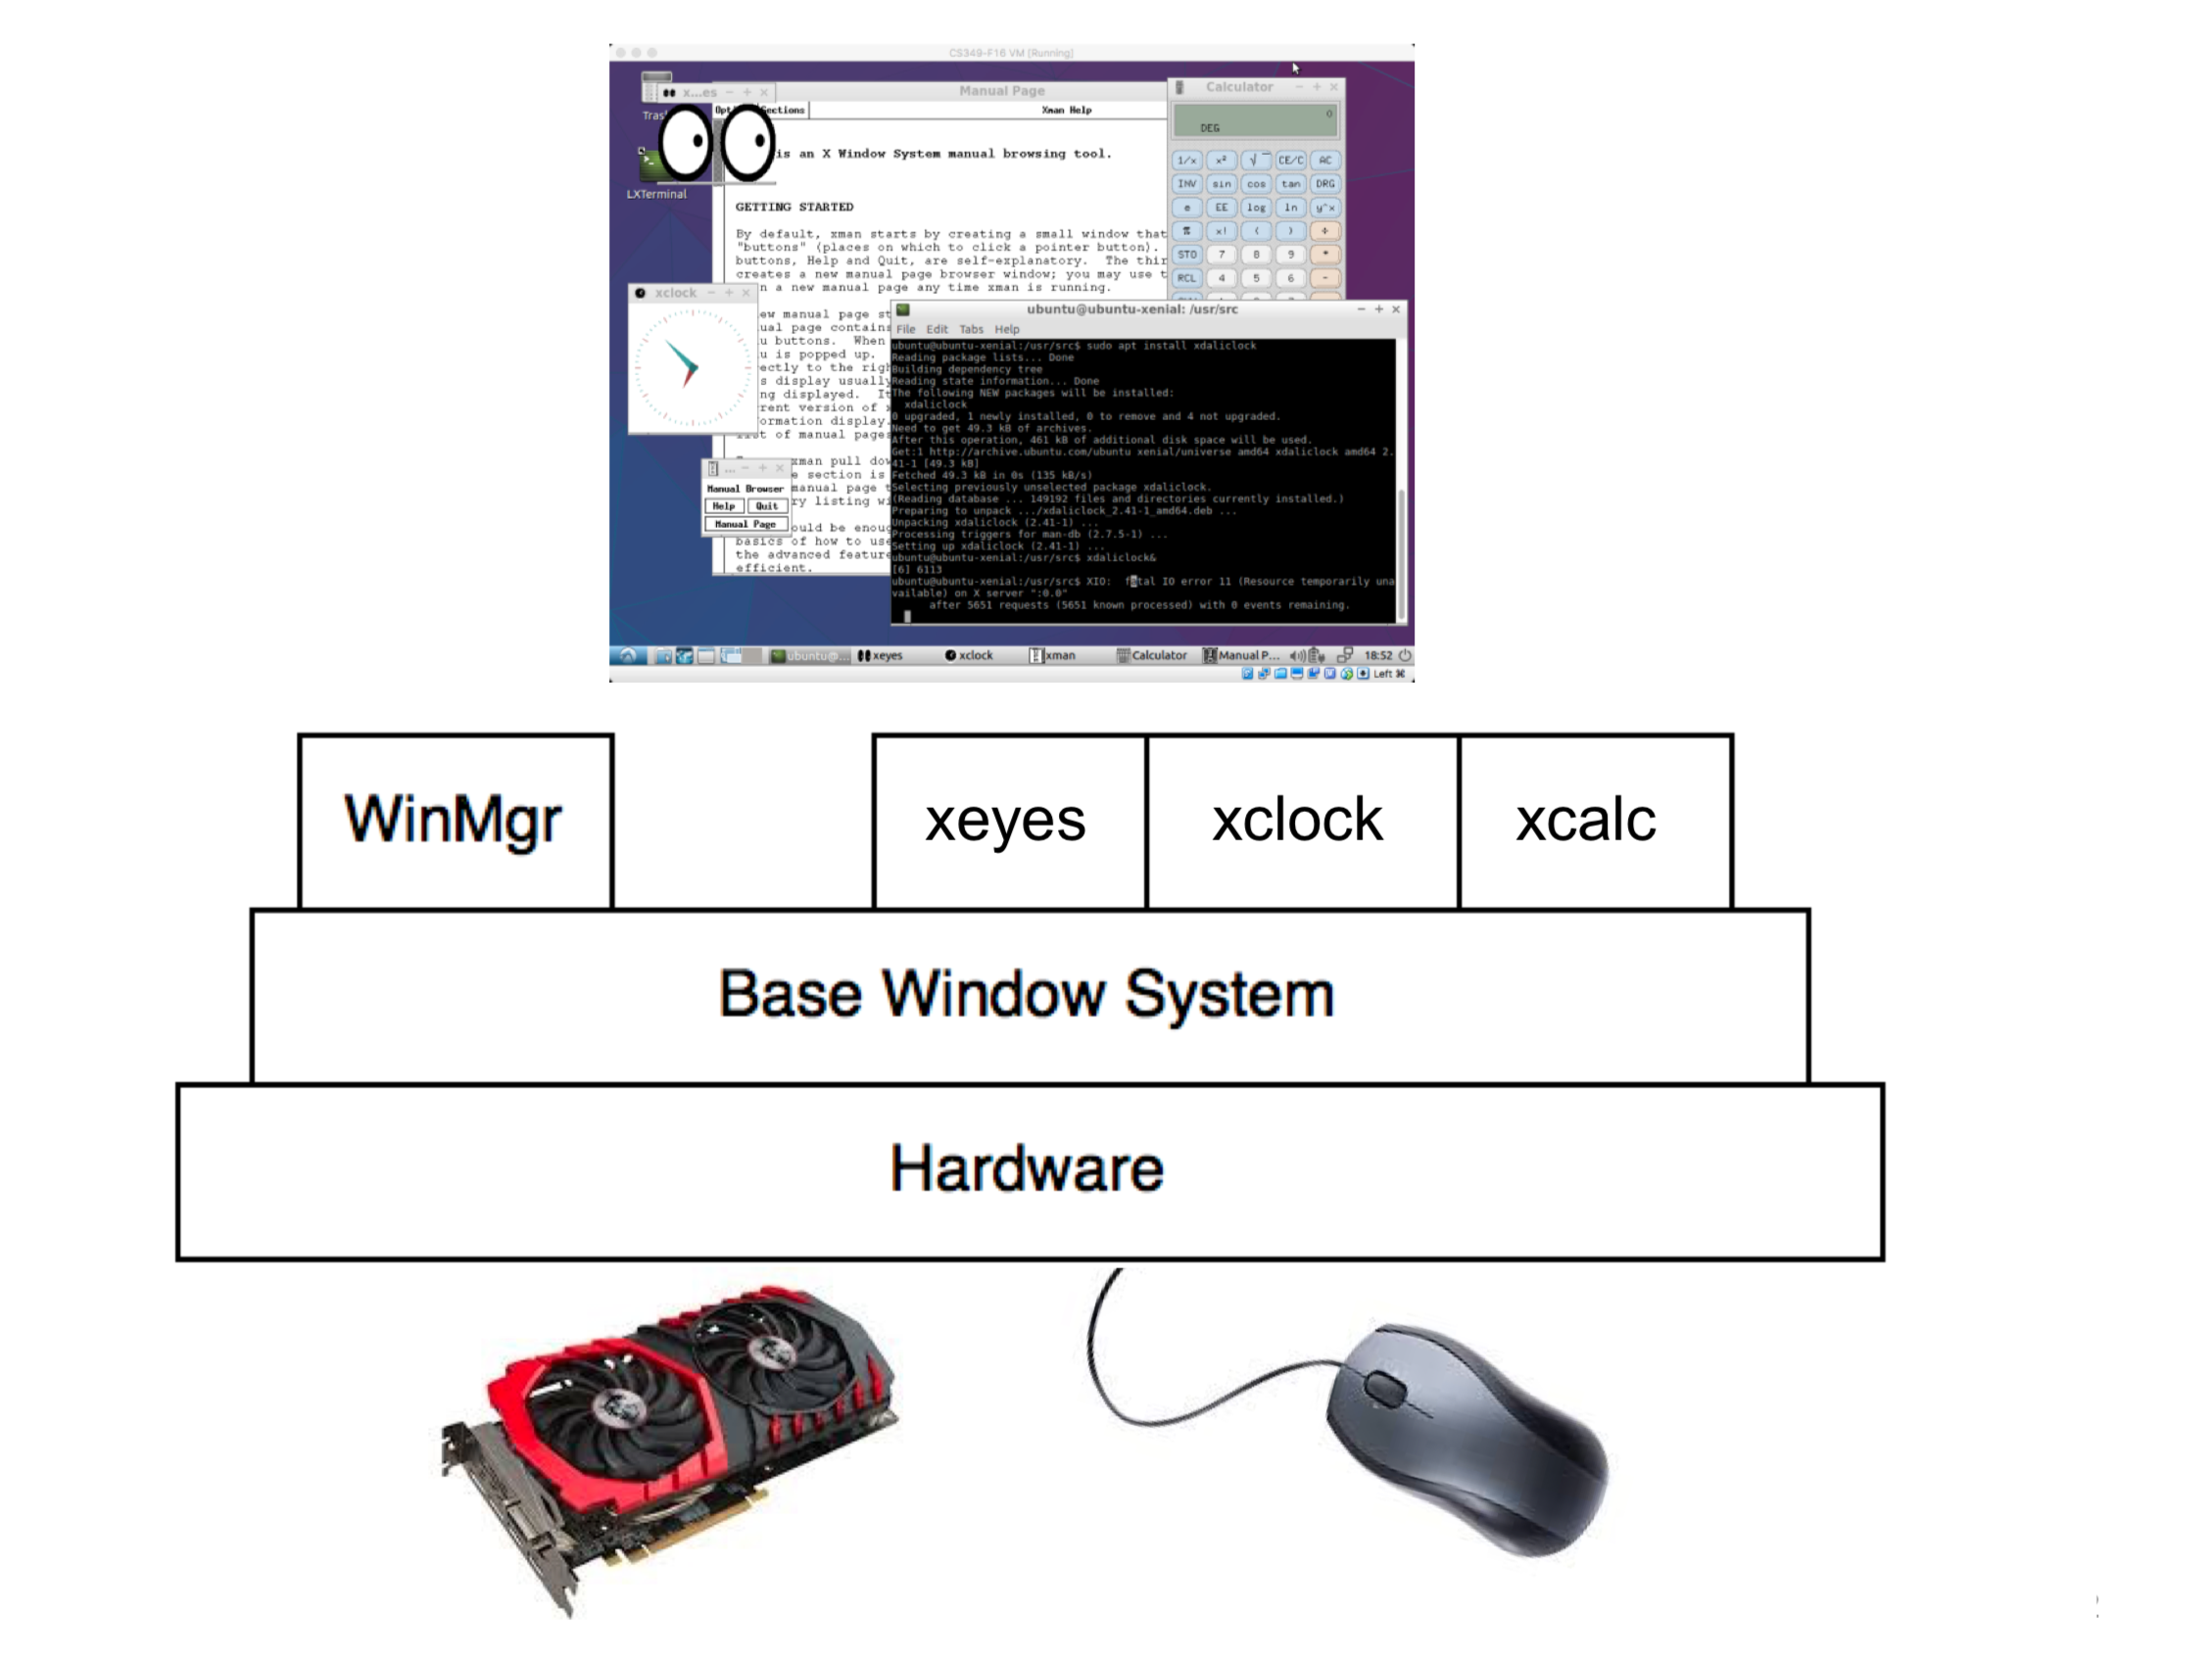
\includegraphics[scale=0.2]{3}
\end{center}

\subsubsection{Base Window System (BWS)}
\begin{itemize}
\item Lowest level abstraction for windowing system 
\item Has routines for creating, destroying, managing windows
\item Also routes mouse and keyboards input to correct window 
\item Ensures only one application changing frame buffer (video memory) at a time
\end{itemize}

\subsubsection{Canvas Abstraction }
\begin{itemize}
\item BWS controls application's access to the window contents using a "drawing canvas abstraction"  
\item The application is shielded from details of frame buffer, visibility of window, and all other application windows
\item Each window has its own coordinate system
\end{itemize}

\subsubsection{Window Manager}
\begin{itemize}
\item Provides interactive components for windows (menus, close box, resize capabilities)
\item Creates the “look and feel” of each window
\item Application ”owns” the contents of the window, but the WM “owns” the application window itself!
\item Separating the BWS from the Window Manager enables : 
\begin{itemize}
\item Alternative “look and feels” for windowing system
\item Different windowing paradigms (i.e. Xmonad for tiled windows)
\end{itemize}
\item Additionally separating the BWS from the Window Manager results in a more robust implementation since BWS and WM are separate processes
\end{itemize}

\end{document}





